\section{Benchmark NIST-1 "Analytic Solution"}
\label{sec:bench-1}

This is the first benchmark problem. Its solution is smooth.
The equation solved is the Poisson's equation.

\begin{equation} \label{poisson}
-\Delta u = f
\end{equation}
in the domain $\Omega = (0, 1)^2$, equipped with Dirichlet
boundary condition given by the exact solution.
The exact solution is $u(x, y) = 2^{4p}x^{p}(1-x)^{p}y^{p}(1-y)^{p}$.
The right-hand side $f$ is calculated by inserting exact solution into (\ref{poisson}).
The solution of NIST-1 is shown in Fig. \ref{fig:sln-nist01}.
Here $p$ is a parameter, determining the polynomial degree of the exact solution.

\begin{figure}[!ht]
\centering
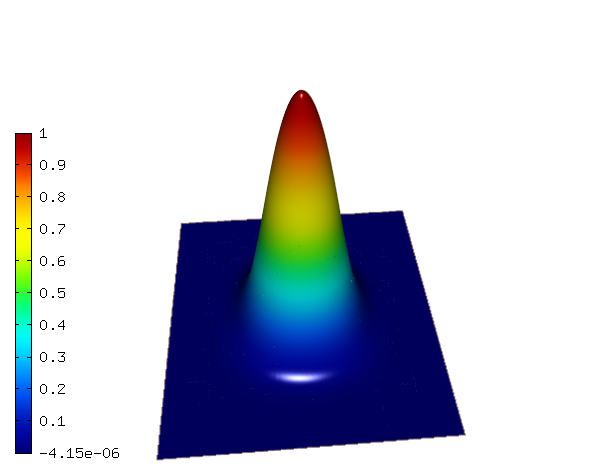
\includegraphics[height=5cm]{nist/nist-1/solution.png}
\caption{The solution to NIST-1 benchmark problem.}
\label{fig:sln-nist01}
\end{figure}

\begin{figure}[!ht]
\centering
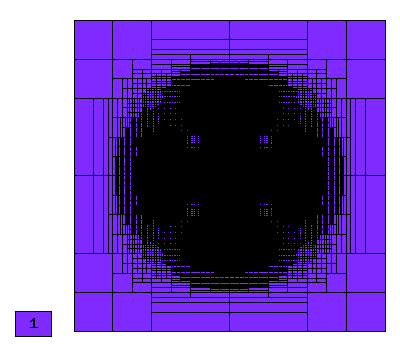
\includegraphics[height=3.7cm]{nist/nist-1/mesh_h1_aniso.png}
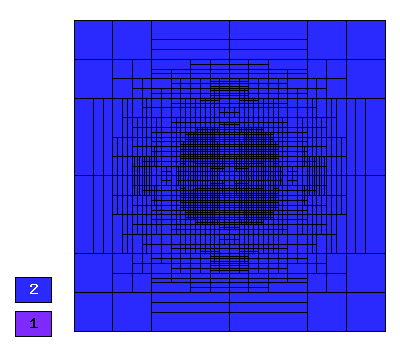
\includegraphics[height=3.7cm]{nist/nist-1/mesh_h2_aniso.png}
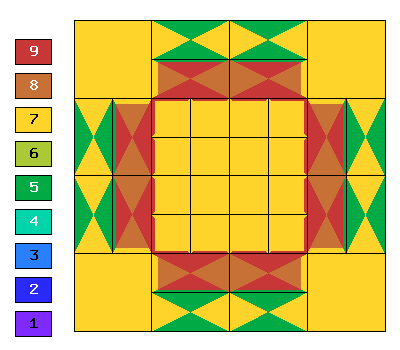
\includegraphics[height=3.7cm]{nist/nist-1/mesh_hp_aniso.png}
\caption{
Final mesh (left) with 51365 DOF and the resulting
relative error estimate in $H^1$-norm of 5.87223e-01 \% for $h$-FEM with linear elements.
Final mesh (middle) with 43401 DOF and the resulting
relative error estimate in $H^1$-norm of 1.37127e-02 \% for $h$-FEM with quadratic elements.
Final mesh (right) with 769 DOF and the resulting
relative error estimate in $H^1$-norm of 4.69543e-03 \% for $hp$-FEM with anisotropic refinements.}
\label{fig:nist-1-hp-aniso}
\end{figure}
%
%\begin{figure}[!ht]
%\centering
%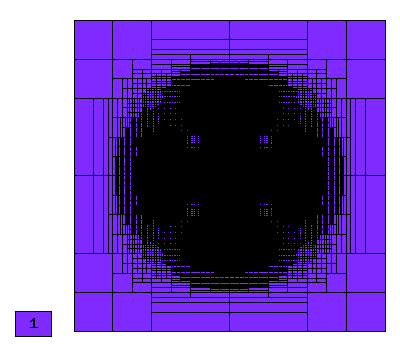
\includegraphics[height=5cm]{nist/nist-1/mesh_h1_aniso.png}\ \
%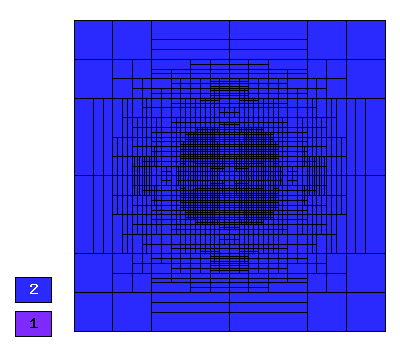
\includegraphics[height=5cm]{nist/nist-1/mesh_h2_aniso.png}
%\caption{Final mesh for $h$-FEM with linear and quadratic elements.}
%\label{fig:nist-1-h-aniso}
%\end{figure}

Figs. \ref{fig:nist-1-conv} compare all
three approaches to automatic adaptivity from the point
of view of DOF and CPU convergence.

\begin{figure}[!ht]
\centering
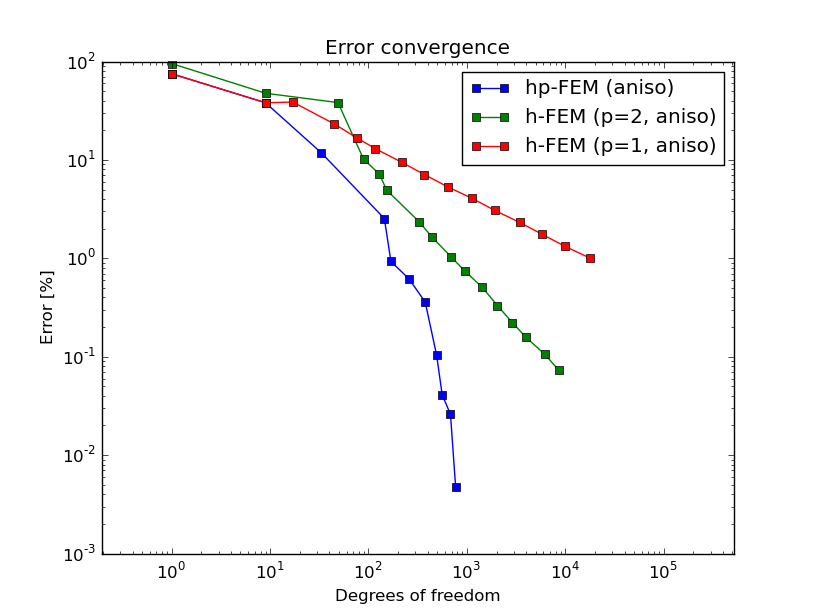
\includegraphics[height=5cm]{nist/nist-1/conv_dof_aniso.png}\ \
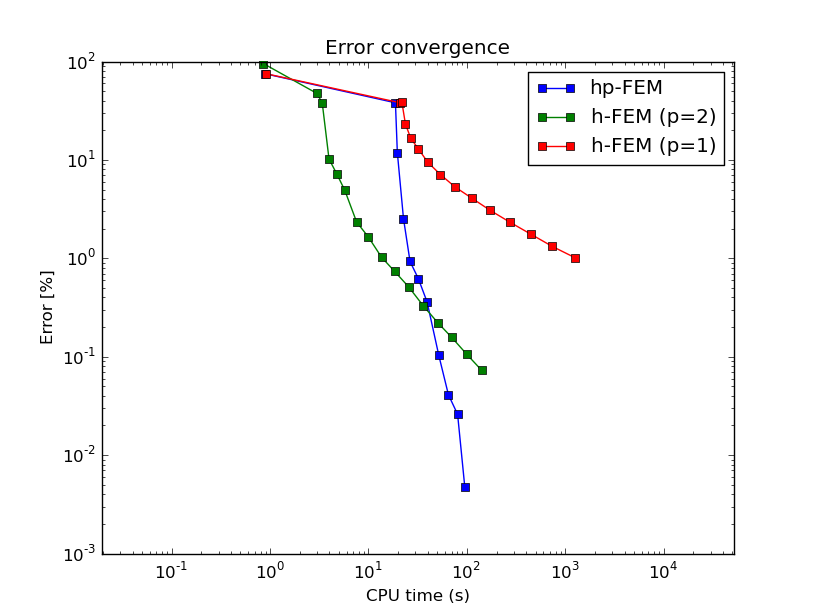
\includegraphics[height=5cm]{nist/nist-1/conv_cpu_aniso.png}
%\vspace{-2mm}
\caption{DOF and CPU time convergence graphs.}
\label{fig:nist-1-conv}
\end{figure}
